\documentclass[aspectratio=169,dvipsnames,svgnames,10pt]{beamer}

\usepackage[T1]{fontenc}
\usepackage[utf8]{inputenc}
\usepackage[french, english]{babel}
\selectlanguage{english}

\usepackage{graphicx}

% Math
\usepackage{amsmath}
% \usepackage{amsfonts}
\usepackage{amssymb}
\usepackage{amsthm}
% \usepackage{mathrsfs}
\usepackage{mathtools}
\usepackage{textcomp}
% \usepackage{textgreek}

% Specialized packages
% \usepackage{syntax} % Grammar definitions
\usepackage{subcaption}
\usepackage{verbatim}
\usepackage{listings} % Code
\usepackage{xspace} % Useful for macros
\usepackage{natbib}% Good citations and bibliography
\usepackage{mathpartir} % Syntax trees
\usepackage{colortbl}
\usepackage{hhline}
\usepackage{multicol}%multicolumn lists
\usepackage{pifont}%% check mark
\usepackage{minted}
\setminted{encoding=utf-8}
\usepackage{wasysym}
\usepackage[normalem]{ulem}% Strike out
\usepackage{multirow}

% \usepackage{mathptmx}
% \usepackage[scaled=0.9]{helvet}
\usepackage{beramono}

\usepackage{natbib}
\bibliographystyle{abbrvnat}

\usepackage{appendixnumberbeamer}

\usetheme{metropolis}
\beamertemplatenavigationsymbolsempty
\setbeamercovered{transparent=20}
\metroset{
  sectionpage=none,
  numbering=fraction,
  progressbar=foot,
}

\def\HUGE{\fontsize{35pt}{15pt}\selectfont}

\title{
  Retrieving library functions by unifying types modulo linear isomorphism\\
  


}
\author{\textbf{Gabriel \textsc{Radanne}}}
\date{}


\begin{document}

\lstMakeShortInline[keepspaces,basicstyle=\small\ttfamily]@

\frame[plain]{
  \centering
  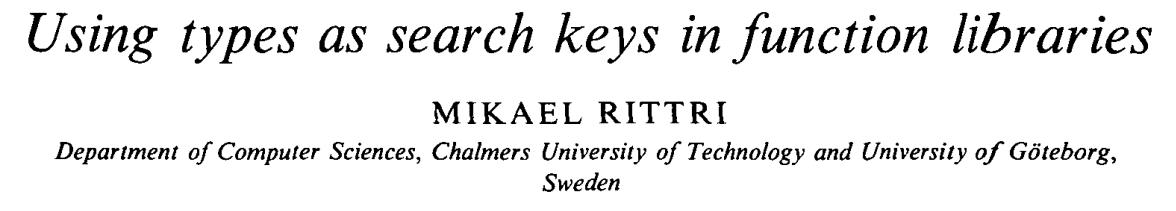
\includegraphics[width=0.9\textwidth]
  {title}
  \vfill
  
\includegraphics[width=0.6\textwidth]{reference1}
  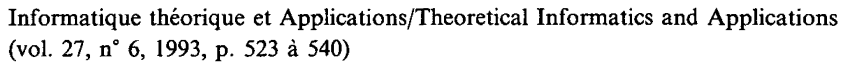
\includegraphics[width=0.7\textwidth]{reference2}
}

\begin{frame}{The beginning}
  Abstract:
  \begin{quote}
    ``A method is proposed to search for an identifier in a functional program library by using its
Hindley-Milner type as a key. This can be seen as an approximation of using the specification
as a key.''
  \end{quote}
\end{frame}

\begin{frame}{Problem}
  Problem, many types are equivalent!

  Example: ``A function to print a real number x with n significant digits.''
  \begin{figure}
    \centering
    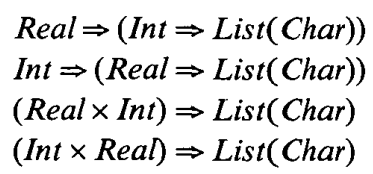
\includegraphics[width=0.4\textwidth]{possibletypes}
  \end{figure}

\end{frame}

\begin{frame}{A solution ?}
  \begin{quote}
    ``What I want, then, is an equivalence relation on types, which abstracts from
    argument order, currying, etc. I could then query a library by giving a type, and get information about all identifiers that have this or an equivalent type.''

    ...

    ``It is natural to say that two types should
be equivalent if it is easy to convert back and forth between them.''
  \end{quote}

  \begin{figure}
    \centering
    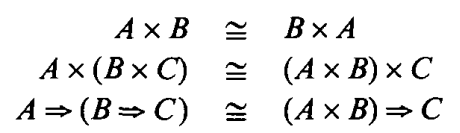
\includegraphics[width=0.4\textwidth]{examples}
  \end{figure}  

  {\small
  (Yes, it's an academic article written in first person. No, don't do that)}
\end{frame}

\begin{frame}
  \frametitle{Definition of isomorphism}

  Correspond exactly to the notion of (mathematical) isomorphisms
  in Cartesian Closed Categories (CCC).
  Fortunately, we don't need categories to define them!
  
  \begin{figure}
    \centering
    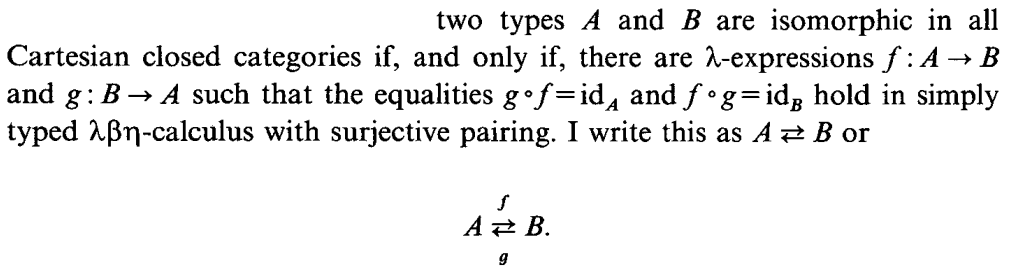
\includegraphics[width=0.95\textwidth]{definitioniso}
  \end{figure}  
  \pause

  $\Rightarrow$ We just need to find a classification !
  
\end{frame}

\begin{frame}
  \frametitle{Classification of all CCC-isomorphisms}
  
  \begin{figure}
    \centering
    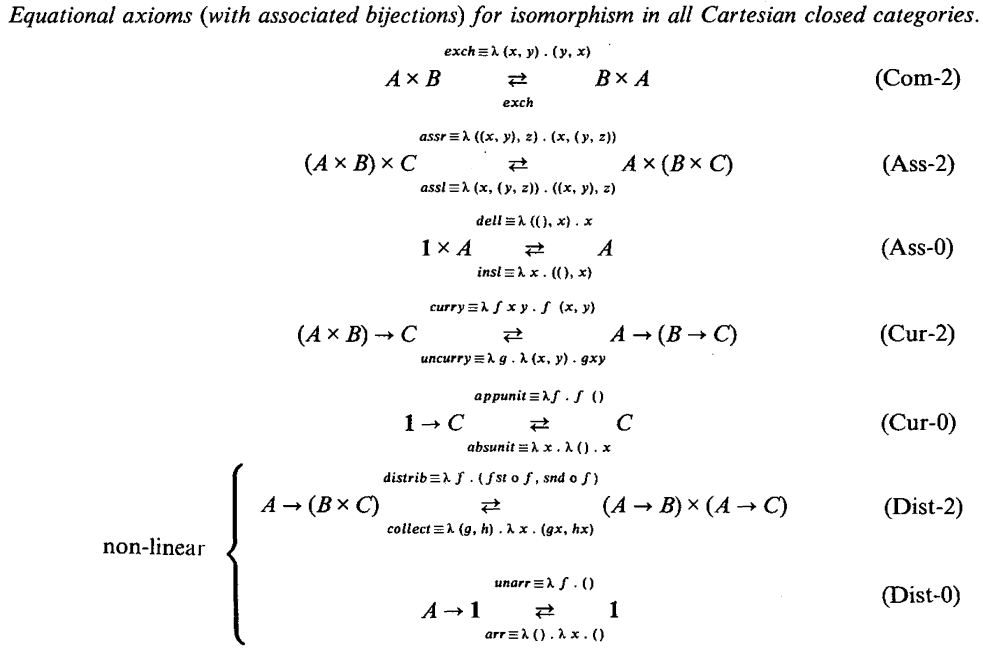
\includegraphics[width=0.8\textwidth]{axiomiso}
  \end{figure}  
\end{frame}

\begin{frame}[fragile]
  \frametitle{What about parametric types ?}

  What if we want to work on a parametric type, for instance, \verb/List(A)/?

  \begin{figure}
    \centering
    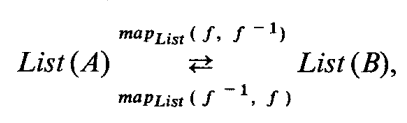
\includegraphics[width=0.4\textwidth]{axiomlist}
  \end{figure}  
  
  $\Rightarrow$ Can be generalized to any free symbol!
\end{frame}

\begin{frame}
  \frametitle{Equational reasoning}

  The isomorphism behave according to our intuition!

  
  \begin{figure}
    \centering
    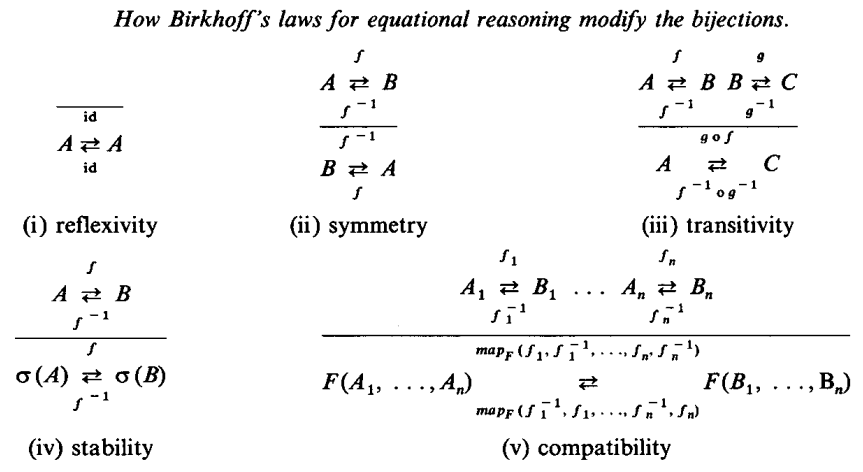
\includegraphics[width=0.7\textwidth]{eqreasoning}
  \end{figure}  
  
\end{frame}


\begin{frame}
  \frametitle{An algorithm for equivalence modulo isomorphism}

  To obtain an algorithm, it is sufficient to orient the rules:
  
  \begin{figure}
    \centering
    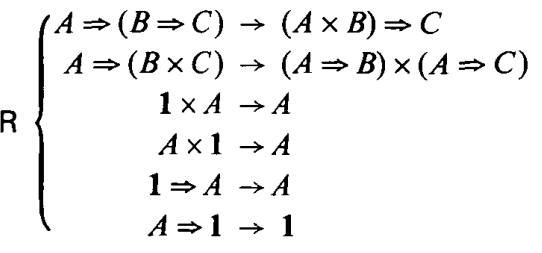
\includegraphics[width=0.5\textwidth]{orientedrules}
  \end{figure}

  We then obtain normal forms, and can use ``bag equality'' (independent of associativity/commutativity).

  The normal forms are exponential with the non-linear axioms!
  
\end{frame}

\begin{frame}
  \frametitle{What about polymorphism ?}

  Recall of some technical terms:
  \begin{itemize}
  \item ``Equivalence'': All variables must correspond, modulo renaming
    \begin{align*}
      \forall A, B.\ A \times B \to A &\cong_{Eq} \forall X, Y.\ X \to Y \to X\\
      \forall A, B.\ A \times B \to A &\ncong_{Eq} \forall Y.\ int \to Y \to int
    \end{align*}
    $\Rightarrow$ This is what we have seen so far.
    
  \item<2-> ``Matching'': Variables can be instantiated {\bf only in one direction}
    \begin{align*}
      \forall A, B.\ A \times B \to A &\cong_{M} \forall Y.\ int \to Y \to int\\
      \forall A.\ A \times int \to A &\ncong_{M} \forall Y.\ int \to Y \to int
    \end{align*}
  \item<3-> ``Unification: Variables can be instantiated {\bf in both directions}
    \begin{align*}
      \forall A.\ A \times int \to A &\cong_{U} \forall Y.\ int \to Y \to int\\
      \forall A.\ A \times list(A) \to A &\cong_{U} \forall Y.\ list(int) \to Y \to list(int)\\
    \end{align*}
  \end{itemize}
\end{frame}

\begin{frame}
  \frametitle{Polymorphism}

  $\Rightarrow$ Unification is the most powerful.

  Some decidability results from the literature
  \begin{itemize}
  \item Equivalence modulo isomorphism is decidable\\
    and as difficult as graph isomorphism
  \item Matching modulo isomorphism is decidable\\
    and NP-complete
  \item Unification modulo isomorphism is undecidable
  \item Unification module \emph{linear} isomorphism is decidable!\\
    and NP-complete
    
  \end{itemize}
  
\end{frame}


\begin{frame}
  \frametitle{Back to practice}
  Rittri implemented everything.

  Example, with a query $\alpha \times Float \to [Char]$
  \begin{figure}
    \centering
    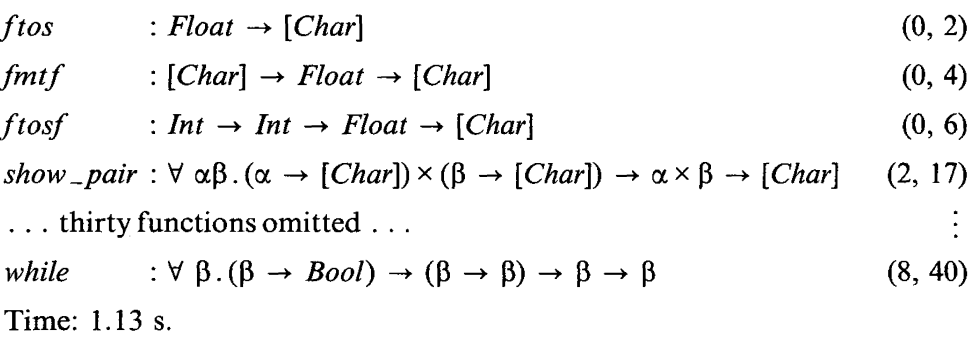
\includegraphics[width=0.8\textwidth]{example}
  \end{figure}
\end{frame}


\begin{frame}
  \frametitle{Very polymorphic query}
  \begin{figure}
    \centering
    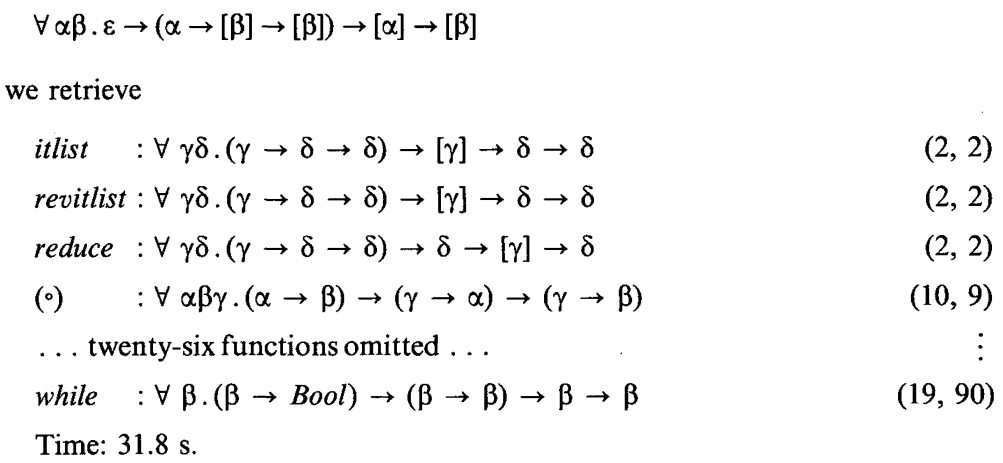
\includegraphics[width=0.8\textwidth]{example2}
  \end{figure}
\end{frame}


\begin{frame}
  \frametitle{Vintage benchmarks!}
  \begin{figure}
    \centering
    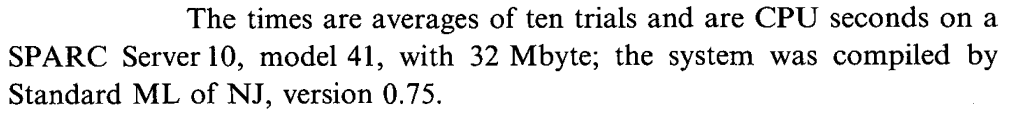
\includegraphics[width=0.9\textwidth]{benchmarks3}
    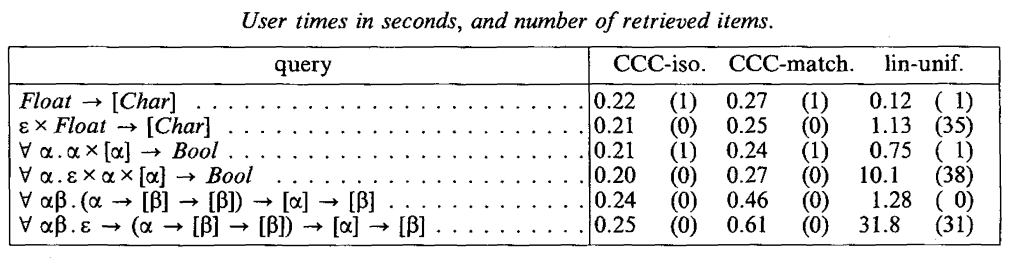
\includegraphics[width=0.7\textwidth]{benchmarks1}
    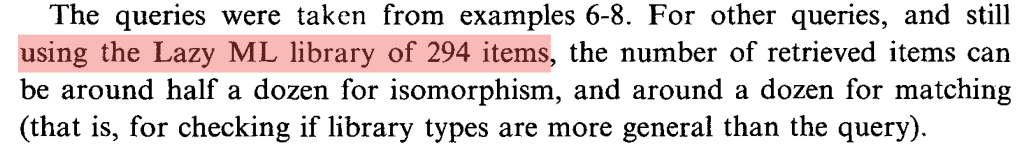
\includegraphics[width=0.9\textwidth]{benchmarks2}
  \end{figure}

  \pause
  $\Rightarrow$ Today's OCaml stdlib is around 2500 functions. It's considered ``very small''. There are 3259 packages in opam. Ecosystems like Typescript are much bigger.
\end{frame}

\begin{frame}
  \frametitle{Conclusion}

  This paper presents a method to search functions in libraries by their types

  $\Rightarrow$ It ignores pesky details, like commutativity and currification,
  thanks to {\bf isomorphisms}.\\
  $\Rightarrow$ Strong theoretical connections with Cartesian Closed Categories
  and unification litterature

  \vspace{2em}

  Since then:
  \begin{itemize}
  \item Lot's of theoretical work to define isomorphism over fancy calculus
  \item Some new and more efficient unification algorithms!
  \item Concept not really applied in practice :(
  \end{itemize}
  
  
\end{frame}

\end{document}

%%% Local Variables:
%%% mode: latex
%%% TeX-master: t
%%% TeX-command-extra-options: "-shell-escape"
%%% End:
